% !TEX root = Hogwarts_1347.tex

\chapter{First Day}

Philippa Laskaris was dreaming of Alexandria.

She was standing on the harbour wall in the late afternoon, the sun behind her, watching the long shadow of the Pharos stretch across the water like a dark finger pointing toward open sea. Her father was beside her, explaining something about currents and shipping lanes, but his voice had acquired a strange, metallic quality --- resonant and rhythmic, growing louder with each word, until the harbour and the lighthouse and the warm Egyptian air dissolved entirely, and there was only the sound.

\textit{Bong.}

She opened one eye.

\textit{Bong.}

The dormitory ceiling came into focus --- high, vaulted stone, crossed by heavy oak beams from which the faded crimson-and-gold banners of Gryffindor hung in long, still drapes. Grey morning light pressed through the tall, narrow windows and lay in pale rectangles across the stone floor.

\textit{Bong.}

The castle bell. She began to count.

\textit{Bong.}

Four.

\textit{Bong.}

Five.

\textit{Bong.}

Six. She pulled the heavy woollen blanket higher, her body making a compelling, well-reasoned argument for remaining exactly where it was. The stone walls held the cold of the night like a cellar, and the warmth beneath the covers was the only civilised temperature in the room.

\textit{Bong.}

Seven.

\textit{Bong.}

Eight.

Eight.

Philippa sat bolt upright, the blanket falling to her waist. Eight bells. Eight bells meant it was almost Terce\footnote{Canonical hours was the medieval system of dividing the day, marked by the number of hours after sunrise. Prime (early morning), Terce (mid-morning), Sext (midday), None (mid-afternoon), Vespers (evening), and Compline (nightfall).}, which meant the morning meal was already half-finished, which meant ---

\enquote{\textit{Merde}. We are late.}

Her voice cut across the dormitory with the flat, unequivocal authority of a girl who had grown up aboard merchant vessels where lateness was measured in lost cargo and strained alliances. She was already swinging her legs over the side of the bed, her bare feet meeting the cold stone with a shock that finished the work the bells had started.

The only other bed in the room was still very much occupied.

Celine Fournier lay on her side, curled beneath her blanket with the total, unreachable commitment of a girl in the deepest trench of sleep. Her dark hair fanned across the pillow in a tangle. One arm hung over the edge of the mattress, her fingers trailing the stone floor. Her breathing was slow, even, and entirely undisturbed by the eight bells, by Philippa's exclamation, or by any sense of urgency the morning might reasonably expect to impose upon a first-year student on her first day of lessons.

Philippa crossed the room in four quick strides and placed a hand on Celine's shoulder.

\enquote{Celine.}

Nothing.

\enquote{Celine. Wake up.}

The girl's breathing did not change. She did not stir, did not shift, did not give any indication that the hand on her shoulder or the voice above her head occupied any part of her consciousness. She slept the way a stone sits at the bottom of a river --- settled, heavy, and profoundly uninterested in the surface.

Philippa shook her, harder this time. \enquote{Celine. It is eight bells. We have missed breakfast. We are going to be late for the first lesson. \textit{Celine}.}

A sound emerged from beneath the hair --- not a word, not quite a groan, but something from the same family. It was the sound of a mind being dragged, against its explicit wishes, toward the waking world.

\enquote{Mmnnhh.}

\enquote{That is not a word. Get up.}

Celine's eyes opened --- slowly, reluctantly, as though the lids themselves were negotiating the terms of their cooperation. She blinked twice at the stone ceiling. Then she turned her head and looked at Philippa, her expression carrying the particular, unfocused bewilderment of a person who has been woken from a dream and has not yet fully accepted the reality she has been returned to.

\enquote{What time is it?} she murmured.

\enquote{Late,} Philippa said, already pulling her robes from the hook on the wall. \enquote{Very, considerably, unacceptably late.}

Celine sat up with visible effort, rubbing her eyes with the heels of her hands. The dormitory came into focus around her. Empty beds. Grey light. Philippa already half-dressed and moving with the controlled urgency of a person who refused to panic but also refused to waste a single second.

Celine pushed the blanket aside and swung her feet to the floor. She reached for her shoes --- placed, as she always placed them, side by side at the foot of her bed.

The left shoe was there. The right shoe was not.

She stared at the empty space for a moment, her still-waking mind processing the absence with the slow, grinding effort of a millstone turning its first revolution of the day. She leaned over the far side of the bed and looked down. Nothing. She ducked her head beneath the bed frame, peering into the dusty shadow between the stone floor and the wooden slats. Nothing. She straightened, frowning, and cast her eye across the floor around the neighbouring beds --- perhaps she had kicked it in her sleep, or it had been nudged aside by one of the other girls on their way out.

It was then that she looked toward the door.

A small, ghostly figure lay across the threshold.

It was a dog --- a terrier, small to medium in build, with the semi-transparent, faintly luminous quality of all Hogwarts spectres. His coat was white, or had been white, rendered now in the pale, pearlescent silver of the dead. He had a scruffy, whiskered muzzle that gave him the appearance of a small gentleman who had neglected to shave, and his ears --- soft and floppy, folded forward at the tips --- framed his face with an expression of guileless, unrepentant mischief. A single black spot marked the left ear, and a second darkened the tip of his tail, the only points of true colour on his otherwise spectral form.

He was lying with his head resting comfortably on Celine's right shoe.

\enquote{Hey, you,} Celine said.

Tawe's tail moved first --- a slow, exploratory wag, as though testing whether the situation warranted the full production. Then his ears lifted, and his dark eyes fixed on hers with the particular, bright intensity of a creature who has been waiting for exactly this moment and is thoroughly delighted that it has arrived.

He rose to his feet. The shoe came with him, clamped gently but firmly in his jaws. He stood in the doorway, holding the shoe with the dignified composure of a retriever presenting a duck, and looked at her.

\enquote{Give me my shoe, please,} Celine said, in the reasonable tone of a girl addressing an unreasonable animal.

Tawe's response was immediate, ancient, and unmistakable. He dropped his front paws flat to the stone, his chest low, his haunches high, his tail beating the air behind him in rapid, joyful arcs. The play bow --- the oldest invitation in the oldest language between the oldest companions. \textit{Chase me. Come and take it. I dare you.}

Celine took a step forward.

Tawe did not wait. He sprang upright, pivoted with a speed that his small frame made almost comical, and bolted directly at the wall. There was no hesitation, no slowing --- he hit the stone at full tilt and passed through it as though it were smoke, the spectral shimmer of his body dissolving into the grey masonry without resistance.

The shoe, which was not a ghost, dropped to the floor with a soft, solid \textit{thud} and lay on the cold stone where the wall met the threshold, very much left behind.

Celine stood still for a moment, looking at the wall. A faint, muffled yip echoed from the other side --- distant already, and self-satisfied.

She picked up the shoe. The leather was still faintly warm where his spectral head had rested on it --- not living warmth, not quite, but a gentle residual heat, like a stone that has sat in the sun and remembers it.

\enquote{Did you see that?} Celine said, pulling the shoe on. A genuine, unhurried smile --- the first of the morning --- spread across her face. \enquote{The little rascal.}

\enquote{You can like him later,} Philippa replied, fastening the clasp of her cloak. \enquote{Move.}

\section*{Bread and Grape Juice}

They moved.

The corridors of Hogwarts in the early morning were not the corridors of Hogwarts at night. The torches burned low in their iron brackets, their flames modest and workmanlike, casting a steady, amber light that lacked the theatrical drama of the evening illumination. The staircases --- which, Cecile had warned them, did not always agree with each other about where they led --- were cooperative at this hour, the stone steps holding their positions with the resigned stillness of structures that had used up their mischief during the night and were now resting.

Philippa set the pace. She moved through the castle with the particular, purposeful stride of a girl who had visited Hogwarts twice before and had committed its principal routes to memory on both occasions --- not from scholarly diligence, but from the practical understanding that knowing where you are going is the first and most important form of power. She took the main staircase down three flights, cut through a tapestried corridor that saved a full minute over the longer route, and descended a final set of wide, shallow steps that opened directly into the entrance hall.

The doors to the Great Hall stood open.

Inside, the four long house tables were still dressed with the remains of the morning meal. Most of the students had already gone --- the benches were largely empty, the conversation reduced to a few scattered clusters of older students lingering over their cups. The enchanted ceiling showed a pale, clean sky streaked with thin cloud, the light falling evenly across the hall, catching the last of the steam rising from the serving vessels.

Philippa's eyes swept the Gryffindor table. The bread baskets were depleted but not empty. The butter crocks had been scraped thin. The fruit --- fresh apples and pears, the last of the shore provisions --- was almost gone entirely, replaced by the honeyed preserves that would carry them through the term. At the far end of the table, a tall clay pitcher of grape juice sat beside a shorter one of barley water, both still a quarter full.

They did not sit down.

Celine reached the table, seized a wooden cup from the nearest stack, and poured the grape juice with the efficient, one-handed motion of a girl who had spent years helping her father serve customers in a bakery where standing still meant falling behind. She drank the cup in three long swallows, standing, her free hand already reaching for a round of dark bread from the basket. The juice was cool and faintly tart, pressed from late-summer grapes, and it cut through the fog of her interrupted sleep with a clarity that no amount of Philippa's shaking had managed.

Philippa moved to the far end of the table, where a clay pitcher of milk still held a few inches. She poured a cup, drank it standing in three measured swallows, and then reached into the fruit bowl. Her fingers closed around a single pear --- the last one, small and slightly bruised on one side but firm --- sitting alone at the bottom of the dish. She took it without comment, the way a merchant's daughter takes the last of anything: quickly, and without drawing attention to the scarcity.

\enquote{Done?} Philippa asked.

Celine tore a large piece from the bread, stuffed it into her cheek, and nodded.

They left the Great Hall at a pace that was not quite a run --- Philippa would not run through the entrance hall; it lacked dignity and attracted attention --- but was close enough to one that the distinction was largely theoretical. Through the entrance hall, past the heavy oak doors, and out onto the broad stone steps that led down to the castle grounds.

\section*{The Lake}
 
The morning hit them like a door opening onto a different world.
 
The air was cold --- properly, unmistakably cold, the kind of Highland autumn air that did not negotiate with clothing but simply went through it. The sky above was enormous, a pale, washed blue that stretched unbroken from the dark line of the mountains in the west to the towers of the castle behind them. The sun was up but still low, casting long shadows across the grass and catching the dew in a million points of white light that made the lawns glitter as though scattered with crushed glass.
 
Before them, the grounds of Hogwarts opened up in a long, gentle slope that ran down toward the lake. The grass was thick and wet, dark green where the shadow still held and bright where the sun had reached it. To the left, the edge of the Forbidden Forest stood like a wall --- dense, dark, and abruptly vertical, the trees pressing together so tightly that the interior was invisible from even a few metres away. To the right, the land rose slightly toward the broom circuit and the distant oval of the arena, whose timber grandstands caught the morning light along their upper edges.
 
But it was the lake that commanded the eye.
 
It filled the lower ground entirely --- a vast, dark, still expanse of water that seemed to absorb the sky rather than reflect it. The surface was black near the centre, where the depth was greatest, and softened to a deep, peaty brown near the margins, where the shallows ran over sand and gravel. The far shore was distant enough that the trees along its edge blurred into a single, continuous line of dark green, and beyond them the mountains rose in long, sweeping ridges, their summits already touched with the first pale dusting of early snow.
 
The group of first-year students was visible halfway down the slope, a loose, colourful cluster of black robes and cloaks moving together toward the water's edge. Philippa and Celine quickened their pace, the wet grass soaking through their shoes as they cut diagonally across the lawn to intercept them.
 
Thomas saw them first. He was walking near the front of the group beside Colum, his broom --- the \textit{Wayfarer}, its dark wood freshly oiled --- resting across his right shoulder. He turned at the sound of their footsteps on the grass and gave them a look that was not quite a smile but occupied the same territory.
 
\enquote{Alive, then,} he said.
 
\enquote{Barely,} Philippa replied, falling into step beside him without breaking stride. \enquote{What did we miss?}
 
\enquote{Porridge. Brown bread. A remarkably aggressive pot of honey that Barnabus nearly dropped into his lap.} Thomas shifted the broom on his shoulder. \enquote{And the announcement that the first flying lesson is by the lake.}
 
Celine, still chewing her bread, looked around the group as they walked. Several of the first-years carried brooms --- new ones, conspicuously so, their handles gleaming with fresh varnish. Laura Orwell carried one as well --- not new, the varnish worn to a smooth, satiny finish along the grip, the stirrup design more refined than the standard student models. It was, Celine guessed, Professor Ligier's.
 
Most of the other students carried nothing.
 
Mæve Medici fell into step beside Celine and Philippa. \enquote{We are going to the lake,} Mæve said. Her tone was informational rather than conversational --- she was reporting a fact, not making small talk. \enquote{The lesson today is by the water. I don't know why. I asked Professor da Senna's assistant, who said only that we should wear clothes we do not mind getting wet.} She paused, considering her own statement. \enquote{I mind getting wet.}
 
\enquote{When did you talk to da Senna's assistant?} Philippa asked.
 
\enquote{At breakfast. He was collecting brooms from the storage shed near the arena. He was carrying a very unusual broom. It was larger than a normal one. It appeared to be built for two riders.}
 
Philippa filed this away without comment. Her eyes had already moved ahead, past the group of students, to the edge of the lake, where the lesson was being assembled.
 
\section*{The Pier}
 
Professor Afonso da Senna stood at the water's margin. He was smaller than Thomas had expected --- shorter than most of the older students, lean and angular, with the tightly wound physique of a person who carried no weight that did not serve a purpose. His dark hair was thick and curly, falling loosely around his face in a way that suggested indifference to grooming rather than neglect. He wore a plain linen shirt beneath a fitted leather jerkin, practical trousers tucked into low boots, and no cloak despite the cold. There was a quality to his stillness that was not relaxation. It was the stillness of a drawn bowstring. The stillness of a man who could move very, very fast and was, at present, choosing not to.
 
Behind him, four older students --- sixth or seventh-years, by the look of them. One of them stood slightly apart, holding between herself and another student a broom unlike any Celine had seen --- significantly longer than a standard model, with doubled foot-supports and a wider, more densely bound tail, built for stability rather than speed. A tandem broom, designed for two riders.
 
To the left of the professor, a wooden rack held perhaps two dozen brooms standing upright in slots. They were not new --- the handles showed the particular, even wear of instruments used by many hands over many terms --- but they were good brooms, well maintained, built to teach properly.
 
But it was the structure on the lake that stopped the group.
 
A wooden pier extended from the shore out over the dark water --- low, solid, and built from heavy, tarred timber. It ran straight for perhaps a hundred metres, its pylons visible through the clear shallows near the bank and vanishing into blackness further out.
 
At the far end, the pier broadened into a wide platform, open on all sides, sitting a foot above the waterline. And on its far edge, a short set of stairs led up to a second, smaller platform --- barely large enough for one person --- from which a single wooden plank projected outward over the open water, unsupported, like a diving board. The plank was perhaps three metres long and it ended abruptly over water deep enough that the bottom was no longer visible.
 
Celine looked at the plank. She looked at the water beneath it. She looked at the brooms on the rack.
 
She looked at Philippa.
 
Philippa was already looking at the plank, and the expression on her face --- the particular, calculating stillness of a girl weighing the available evidence and arriving at a conclusion she did not entirely enjoy --- confirmed that they were both thinking the same thing.
 
Mæve, who had been reading her book throughout the entire walk and had only now looked up to take in the scene, closed the volume with a slow, deliberate motion.
 
\enquote{I mind getting wet,} she said again, very quietly.
 
\section*{First Flight}
 
Da Senna let them arrive. He did not call out, did not wave them over, did not hurry the stragglers. He simply waited, hands at his sides, until the group had gathered in a loose, uncertain semicircle around him at the water's edge, and then he smiled --- a brief, warm thing that softened the brooding architecture of his face entirely --- and said, \enquote{Good morning.}
 
His Latin was crisp and lightly accented, carrying the rounded vowels of Portuguese beneath the formal grammar.
 
\enquote{Those of you who brought your own brooms, keep them. The rest of you --- take one from the rack.}
 
Students selected brooms with varying degrees of confidence --- some lifting them from the rack with practised ease, others holding them at arm's length as though they might bite.
 
Da Senna picked up his own broom --- a lean, dark instrument that seemed to resent any gram of unnecessary weight --- and nodded toward the pier. \enquote{Follow me.}
 
They walked the length of it in a loose procession, the wooden planking solid and wide beneath their feet, the loch opening up around them as they moved further from the shore. The water below darkened steadily, turning black and depthless by the time they reached the broad platform at the pier's end.
 
When they had assembled, da Senna held his broom in front of him.
 
\enquote{Place the broom between your legs,} he said. He demonstrated, tucking the shaft beneath him. \enquote{Your body should sit as close as possible to the broom's centre --- the point where the weight of the handle ahead of you and the weight of the tail behind you are in balance. You will feel it. When you are in the right position, the broom will feel light.}
 
He watched as twenty-odd first-years arranged themselves. Philippa found her balance quickly. Mæve did not. Julian looked down at himself and seemed more concerned with whether the position looked right than whether it was.
 
\enquote{Your hands,} da Senna continued. He placed his right hand forward on the shaft, his left behind it, both grips firm but not white-knuckled. \enquote{Right hand leads. It controls the inclination of the nose --- tip it down to accelerate, tip it up to slow or climb. Your left hand steadies and firms the position. Hold it firm. Do not squeeze, there's no need.}
 
He paused. \enquote{For those of you who are left-handed, reverse the grip. Left leads, right steadies.}
 
Thomas adjusted. Across the platform, Laura Orwell had already done so.
 
\enquote{Now --- the legs.} Da Senna pressed his calves inward against the shaft. \enquote{The broom is not a chair. You do not sit upon it. You hold it with the whole of your lower body --- thighs, knees, calves. The tighter your legs, the more control you have in turns. But for now, just feel the position. Walk with it. Let your body learn where the broom wants to be.}
 
He stepped off the platform and walked a short loop along the pier, the broom tucked between his legs as naturally as a sword in a scabbard. The students followed, a procession of slightly bow-legged first-years shuffling along the wooden planking with their brooms clamped beneath them, looking --- Thomas thought --- considerably less glamorous than any of them had pictured themselves.
 
When they had returned to the platform, da Senna mounted a small wooden box that one of his assistants had placed near the edge. He was still holding the broom between his legs, his posture unchanged.
 
\enquote{The nose,} he said, tilting the front of the broom upward with his right hand. \enquote{Fifteen degrees above level --- this is your departure angle. It gives you lift and forward motion together. From a standstill, this is how you begin.} He adjusted. \enquote{Flatten the angle and you go faster. Steepen it and you slow down, or climb. If you want to stop --- pull up until the broom is level or slightly above, and let the speed bleed away.}
 
He looked at them. \enquote{The best way I can describe what you are about to do is this: flying a broom is like falling forward and never reaching the ground. You keep a slight upward inclination so that you are, at the same time, rising and falling --- the two cancel each other, and the result is a straight line through the air.} He let that settle. \enquote{It sounds complicated. It is not. Your body will understand it faster than your mind will. Trust the fall.}
 
And then, without ceremony, he stepped off the edge of the box.
 
The broom caught him. He rose perhaps a metre above the platform, drifted forward over the dark water, banked left in a turn so sharp and clean that the tail of the broom drew a visible line in the morning mist, and came back. He dismounted onto the platform with unhurried precision.
 
The whole thing had taken perhaps five seconds.
 
\enquote{Now,} he said, and his smile returned. \enquote{The fun part.}
 
He walked along the line of students, making small adjustments as he went --- a hand repositioned here, a grip loosened there, a broom shifted an inch forward on a boy who had been sitting too far back. His corrections were quick and physical, a touch on the wrist, a tap on the knee, rarely more than a word or two. When he reached Hector Hawthorne, who was holding his ash-handled broom with absolute confidence, da Senna stopped. He looked at the boy's grip, his posture, the angle of the shaft --- all of it held with unshakeable certainty. Da Senna reached forward, moved Hector's right hand two inches down the shaft, pressed his left elbow inward, and shifted the broom's position against his legs. Hector's expression tightened, but he said nothing.
 
When he was satisfied, he directed them toward the stairs of the elevated platform. \enquote{Form a line. One at a time. Walk to the end of the plank, set your angle, and jump.}
 
He pointed toward the water, where a wooden buoy floated roughly a hundred and fifty metres from the platform, painted bright red and bobbing gently on the still surface. \enquote{Your target is the buoy. Fly to it, circle it, and return here. You will not reach it on your first attempt. That is expected.} He gestured toward the two older students who now sat mounted on the tandem broom, hovering just off the edge of the platform with the unhurried competence of a pair who had done this dozens of times. A third assistant hovered nearby on a single broom. \enquote{When you fall --- and you will fall --- they will collect you. The water is cold but you will not be cold for long.}
 
He looked at the fourth assistant --- a young blonde Gryffindor who stood on the main platform holding her wand. \enquote{Miss Ashworth will take care of that.}
 
She nodded.
 
Da Senna stepped aside.
 
For a moment, nobody moved. Twenty-odd first-years looked at the plank, looked at the water beneath it --- black, still, and entirely indifferent to their feelings about the situation --- and then looked at each other.
 
Ewan MacIntyre broke the silence by walking to the front of the line with a determined stride --- hesitation was a problem best solved by not engaging in it.
 
He climbed the five stairs. The elevated platform was small --- barely enough room for one person and a broom --- and from up here the perspective changed. The main deck below looked further away than it should have. The pier stretched back toward the distant shore like a long, thin arm. And ahead, the plank extended over nothing, its rough surface ending in open air above water that was very deep and very dark.
 
Ewan walked to the end of the plank. It flexed slightly beneath his weight. Below him, the loch waited still.
 
He set the angle of his broom. Fifteen degrees.
 
He jumped.
 
The broom caught the air and surged forward --- faster than he had expected, the acceleration immediate and startling, the wind pressing against his face and chest with a force that made his eyes water. The platform fell away behind him. The water rushed beneath, dark and close, the surface blurring with speed. For perhaps half a second he was flying --- genuinely, unambiguously flying --- the broom humming beneath him, the loch enormous and glittering and impossibly open.
 
Then the nose dipped.
 
The descent was not dramatic. It was the gentle, inevitable surrender of a broom whose rider did not yet know how to sustain the angle --- a slow forward tilt, the tail rising, the water coming up to meet him with a calm that felt almost polite. Ewan had enough time to think \textit{well, that was more than I expected} before the surface hit him, a shocking, full-body cold that drove the breath from his lungs and filled his ears with a muffled roar.
 
He surfaced, gasping, his hair plastered flat, his broom floating beside him.
 
Twenty metres. It was, as first flights go, a very respectable distance.
 
The tandem broom was beside him within seconds, one of the pilots leaning sideways with a practised, extended arm. \enquote{Grab the shaft --- like a branch. Both hands. Up you come.}
 
The solo flyer retrieved Ewan's broom from the water and carried it back to the platform. Ewan arrived a moment later, dripping copiously, his grin suggesting that the cold had not remotely dampened his enthusiasm.
 
Gale Ashworth was already waiting. She raised her wand.
 
\enquote{\textit{Calefacio}.}
 
The cold left him like a retreating tide --- the chill in his bones, the ache in his fingers, the sharp bite in his chest --- all of it replaced by a spreading, deeply pleasant warmth that started at his core and moved outward until even his soaking shoes felt comfortable. Small plumes of vapour rose from his robes.
 
\enquote{\textit{Exsicca vestimenta}!}
 
The water vanished from his clothes in a matter of seconds, the fabric going from dark and heavy to light and dry with a speed that felt faintly miraculous. Ewan looked down at himself, entirely dry, entirely warm, and let out a laugh.
 
\enquote{That,} he said to no one in particular, \enquote{was brilliant.}
 
Philippa was next. She set her angle with care, jumped cleanly, held the line for a long, promising stretch, and then over-corrected a slight drift to the left, the broom rolling sideways and depositing her in the loch with a splash that was, by the standards of the morning, almost graceful. Eighteen metres.
 
Celine followed. She stood at the end of the plank for longer than Philippa had, looking not at the water but at the sky above it, and when she jumped her face held an expression of pure, reckless delight that lasted precisely until the broom began to descend, at which point it was replaced by an expression of pure, reckless alarm. Twelve metres. She came back to the platform laughing so hard that Gale had to wait for her to hold still before casting the drying charm.
 
Thomas's first attempt was short and violent. He launched well --- the broom leapt from the plank with a force that drew a murmur from the students watching --- but his grip was too tight, his correction too sharp, and the \textit{Wayfarer} pitched sideways and dumped him after barely ten metres. He surfaced, shook the water from his hair, and said nothing. On his second attempt, he made twenty-five.
 
Cassian Sterling jumped while looking up. It was not clear whether this was deliberate or simply the natural consequence of being Cassian Sterling, but the result was a surprisingly stable flight --- eyes on the horizon rather than the water beneath --- that carried him a respectable distance before ending in the usual manner. He emerged from the loch with perfect calm, as though the experience were an interesting data point rather than a personal failure.
 
The rounds continued. Each attempt was longer than the last --- not always for the same student, but collectively, the average crept upward. Brooms stayed airborne for five seconds, then eight, then twelve. The falls became less dramatic, the corrections less wild. A rhythm established itself: the climb, the walk, the jump, the flight, the splash, the rescue, the warmth. The \textit{Calefacio} charm began to feel less like first aid and more like a small, earned comfort --- the warm handshake at the end of an honest effort.
 
Ashworth, who had begun the morning performing the spells with brisk, professional efficiency, was smiling by the tenth student. By the twentieth, she was applauding with the rest of them.
 
Edmund Varre, on his third attempt, reached the buoy.
 
The platform went quiet as he approached it, his broom steady, his angle good, the red-painted wood growing larger in front of him. He passed it on the left side, began the turn --- and the broom's tail swung wide, the radius too tight, his weight shifting to the outside of the curve. The correction came too late. He slashed sideways across the surface, throwing a spectacular arc of spray, and his wand flew from his hand and landed in the loch a good twenty metres from where he surfaced.
 
He came back to the platform without the wand. One of the solo flyers retrieved it a minute later, dripping. Edmund accepted it, wrung the water from his sleeve, and said, with quiet dignity, \enquote{The turn needs work.}
 
Barnabus Finch was, in most respects, an unlikely candidate for the first completed circuit. The round-faced boy was not particularly athletic, and his first two attempts had ended in splashes that were enthusiastic in their volume if modest in their distance. But on his fourth try, something settled. His grip was easy, his angle steady, and when the buoy came he took it wide --- a gentle, sweeping arc rather than a sharp turn, the broom banking smoothly, the tail holding its line.
 
He came around the far side. The broom straightened. He was heading back.
 
The platform went silent. Not the held-breath silence of tension, but the watching silence of a group that has just realised something is about to happen.
 
Barnabus crossed the distance in a clean, unwavering line. His speed was modest --- he was not fast, and did not try to be --- but the flight was steady, balanced, and entirely under control. The platform grew larger ahead of him. The faces of his classmates grew distinct.
 
He landed on the wooden deck with a soft thud, both feet finding the planks, the broom still humming beneath him.
 
Dry.
 
For a single, suspended moment, nobody moved.
 
Then the platform erupted. The sound was enormous --- cheers, whistles, stamping feet that made the wooden structure shake --- and Barnabus stood in the middle of it looking slightly stunned, as though he had not entirely decided whether to be proud or embarrassed and had settled, for the moment, on a combination of both that manifested as a very wide, very red-faced grin.
 
Da Senna, standing at the edge of the platform, brought his hands together three times --- quiet, measured claps that carried no less warmth for their restraint.
 
Cassian Sterling completed the circuit shortly after, his line steady and his gaze, characteristically, fixed on a point somewhat above the practical horizon. After that, the thing that had been impossible became merely difficult, and then achievable, and then --- one by one, round by round --- achieved. Each returning student was met with cheers that grew louder and less surprised and more purely joyful as the morning wore on, the applause of a group that had discovered it was capable of something it had not been capable of an hour ago.
 
Colum made it look easy when his turn came --- his flight clean and grounded, his turn around the buoy taken at a sensible radius, his landing on the platform accompanied by a modest nod that drew, inevitably, the loudest cheer of the morning, which turned his face the colour of a ripe apple.
 
Thomas's fifth attempt was the one that worked. The \textit{Wayfarer} moved differently when he stopped fighting it --- the dark wood responsive and alive beneath his hands, the broom's natural balance finding his own. He took the buoy at speed, the turn sharper than Barnabus's but controlled, the loch blurring beneath him, and returned to the platform with his pale hair --- he had not noticed the shift --- catching the late morning sun.
 
\enquote{Well done,} da Senna said. \enquote{Very well done, everyone.}
 
He waited for the last of the cheers to subside, then raised his voice. \enquote{But anyone can fly forward. More tricky is to hover still.}
 
He mounted his broom, rose a metre from the deck, and held his position --- perfectly, absolutely motionless --- as though the air beneath him had solidified into glass. The broom did not drift. He did not sway. He simply hung there, still and patient, the loch stretching out behind him.
 
\enquote{Hovering,} he said, from his position in the air, \enquote{is what happens when you fly forward slower and slower until you stop. You keep the balance. You keep the slight inclination. But you let the speed fall away until there is none, and then --- you stay.}
 
He descended and looked at the class. \enquote{Who would like to be first?}
 
Twenty voices answered at once, a chorus of high-pitched, eager shouts that collided in the cold air and became a single, indistinguishable noise of enthusiasm. Da Senna's expression suggested he had expected precisely this.
 
He pointed at Barnabus. \enquote{Mr. Finch. Fly toward the buoy. Halfway there, begin to raise the nose --- gently, slowly --- and let yourself decelerate until you are still.}
 
What followed was, by any objective measure, a catastrophe --- but it was a catastrophe conducted in excellent spirits.
 
Barnabus launched well, pulled up too sharply, and the broom reared beneath him like a startled horse, tipping him backward into the water. Philippa attempted a gradual slowdown and drifted sideways off the broom instead, describing a slow, almost peaceful arc into the loch. Thomas, overcompensating again, sent the \textit{Wayfarer} shooting forward out from under him when he pulled up --- the broom sailed nearly to the buoy before one of the assistants caught it, while Thomas dropped vertically into the water with a directness that at least had the merit of efficiency.
 
Cassian stalled beautifully but forgot about lateral drift and tipped sideways. Julian achieved something close to a hover for two full seconds before a gust of wind --- barely enough to stir a flag --- dislodged him with a yelp. Celine decelerated smoothly, stopped, hung in the air for one radiant, astonished heartbeat, and then burst out laughing, which broke her concentration entirely and dropped her straight down.
 
The \textit{Calefacio} charm flowed like wine. Gale's wand arm must have ached, but her smile did not falter.
 
Da Senna watched from the platform with his arms folded, quietly satisfied --- everything was unfolding exactly as he had expected. The older student assistants, who had spent the morning in professional, efficient silence, had by now abandoned all pretence of detachment and were cheering alongside the first-years after every attempt.
 
Laura Orwell was the first to hold it.
 
She flew out, decelerated in a smooth, continuous curve, and stopped. The broom hung motionless above the dark water, Laura's body perfectly still, her balance absolute. She held the position for five seconds, then ten, the only movement the faint stirring of her dark hair in the wind off the loch. Then she turned, flew back, and landed on the platform without a word.
 
Elara succeeded not long after, her hover slightly lower and slightly less steady than Laura's but held with a calm, focused stillness that seemed to come from the same place as her art --- a patience for the thing in front of her, a willingness to wait until it was right. Celine followed, finding the balance she had lost to laughter on her previous attempt, and this time she did not laugh --- she simply hovered, her face bright with a quiet, private wonder, and the cheers that met her return were warm and real.
 
After that, the dam broke. One by one, the first-years found the stillness --- some quickly, some after five or six more rounds of trying --- and each success was met with the same noise, the same stamping and clapping and whistling that shook the wooden platform and carried out across the still surface of the loch.
 
The sun sat higher in the sky by the time da Senna raised his hand.
 
\enquote{That is enough for today.}
 
The cheering subsided, though the energy did not --- it hummed in the group like a plucked string, the residual excitement of a morning that had delivered more than any of them had expected.
 
Da Senna called the first-years to gather around him. He stood with his broom held loosely at his side, his expression warm but not effusive --- genuinely pleased and seeing no reason to exaggerate the fact.
 
\enquote{You have done very well,} he said. \enquote{All of you. A very good first class.}
 
He let the compliment land, then continued. \enquote{I have instructed one of my assistants to be present by the lake each day between prime and terce. If you wish to practise your flight outside of class hours, I encourage you to do so.} His expression sharpened, just slightly. \enquote{But flying over the lake without supervision is strictly forbidden for all first-years. This is not a suggestion.}
 
He looked at them --- twenty-odd flushed, wind-bitten, slightly damp faces looking back at him with the bright, undivided attention of children who had just discovered something extraordinary about the world and about themselves.
 
\enquote{There are more than wands in the wizarding world,} he said.
 
He picked up his broom, tucked it under his arm, and walked back down the pier toward the shore, his assistants falling into step behind him.
 
The group dispersed slowly, in the way that groups do when no one quite wants the thing to be over. Some lingered on the platform, talking in twos and threes, replaying their flights with the breathless, overlapping narration of the recently amazed. Others started the long walk back up the slope toward the castle, their brooms over their shoulders or dragged along the grass behind them.
 
Celine walked beside Philippa, her shoes squelching faintly and her face still carrying the afterglow of the morning. She tilted her head back and looked at the sky, pale and enormous above the mountains, and smiled at nothing in particular.
 
\enquote{I want to go again,} she said.

\section*{The Gambeson}
 
The message arrived during lunch --- a folded slip of parchment, passed down the Gryffindor table by a prefect who had received it from a second-year who had received it from a house-elf who had received it from nobody could say. The instruction was brief: all first-year students were to report to the Defence Against the Dark Arts classroom on the third floor immediately following the meal. No further explanation was given.
 
\enquote{That's odd,} Reza said, reading over Thomas's shoulder. \enquote{Defence isn't until None.}
 
\enquote{So why do they want us there early?} Colum said.
 
\enquote{I suppose we'll find out,} Philippa said, folding her napkin with unhurried composure.
 
They climbed the stairs to the third floor in a loose, mixed procession --- Gryffindors, Hufflepuffs and Ravenclaws converging from different staircases, a few Slytherins already ahead of them, moving with the wary curiosity of students summoned without context. The corridor was wide and well-lit by tall, narrow windows that let in the pale afternoon light and a persistent draught.
 
The Defence Against the Dark Arts classroom was large --- larger than Thomas had expected, and sparer. The ceiling was high and vaulted, crossed by heavy stone ribs, and the walls were bare grey masonry broken only by the windows and a series of iron sconces holding unlit torches. There was very little decoration. A row of padded training dummies stood against the far wall, their surfaces scarred and scorched from years of spell practice. Beside them, a set of anatomical diagrams --- detailed, clinical illustrations of spell damage to human tissue --- hung from iron hooks, their parchment yellowed but their content unpleasantly vivid. Two heavy oak desks sat at the front of the room, and the student benches were arranged in a wide semicircle facing them. It was not a room that believed in comfort. The things taught here were not comfortable, and pretending otherwise would be a disservice to the children who needed to learn them.
 
Professor Ligier was not in it.
 
Instead, standing behind the oak desks with a knotted cord of measuring rope around his neck and a leather roll of tools spread open before him, was a man in his fifties --- tall, with the rolled sleeves and chalk-dusted fingers of a working tradesman. Beside him stood a young woman, perhaps twenty, who shared his blunt features and the same measuring rope around her own neck. Between them, a charmed quill floated above each of two open notebooks, poised and ready.
 
\enquote{Come in, come in,} the man said, beckoning the students forward. \enquote{Don't linger in the doorway. Find a place to stand. My name is William Taylor, and this is my daughter Catherine. We are here to take your measurements.}
 
The students filed in, exchanging glances. A tailor. They had climbed three flights of stairs to meet a tailor.
 
\enquote{Arms out to the sides, please,} Taylor said. \enquote{Chin level. One at a time, starting from the left.}
 
He did not wait for questions. The moment the first student --- Ewan, who had positioned himself at the front of the line because hesitation was never his preferred approach --- extended his arms, the two measuring ropes leapt from their owners' necks and flew. They moved with startling speed and independence, one snaking around Ewan's shoulders and chest while the other dropped to his waist and hips, cinching and releasing in rapid succession. Behind the Taylors, both quills scratched furiously, recording numbers onto the floating notebooks in a quick, dense hand.
 
The ropes moved to the next student, and the next. The process was fast --- barely a minute per person --- and the tapes brooked no resistance. When Celine flinched as the rope whipped around her ribs, Catherine Taylor said, without looking up, \enquote{Breathe normally. It knows what it's doing.}
 
\enquote{Does it have to know so aggressively?} Celine muttered, holding still.
 
When the last student had been measured, William Taylor gathered both ropes with a practised flick of his wrist. They coiled themselves neatly around his forearm.
 
\enquote{Your house uniforms --- shirts, trousers, dresses, robes, cloaks, hoods and greatcoats, in your respective house colours --- will be ready in approximately one week,} he announced. \enquote{Until then, your plain black uniforms will suffice.}
 
\enquote{Now,} he said. \enquote{The fun part, if you please, Catherine.}
 
Miss Taylor stepped to the side of the room, where four large trunks sat on a heavy table. Each trunk was marked with a distinct emblem --- the lion of Gryffindor, the serpent of Slytherin, the eagle of Ravenclaw, the badger of Hufflepuff --- and when she unlatched them one by one, the lids swung open to reveal dense, carefully folded stacks of gambesons. Several colour combinations sat within each trunk, all following the palette of their respective house, the quilted fabric thick and professional.
 
\enquote{One each,} Miss Taylor said. \enquote{Find your house trunk and select your preference.}
 
The students moved forward. Thomas reached into the Gryffindor trunk and lifted out a gambeson. He held it up by the shoulders.
 
It was enormous.
 
The sleeves hung a full two feet past his fingertips. The hem would have reached his shins. The shoulders were broad enough for a grown man, and the padded bulk of the thing made it look less like a garment and more like a piece of furniture.
 
Around the room, the same realisation was spreading. Philippa held hers at arm's length and looked at it the way a merchant inspects goods she suspects are defective. Conall turned his over in his hands with quiet confusion. At the Hufflepuff trunk, Barnabus had unfolded his fully, and it pooled on the floor around his feet like a collapsed tent.
 
\enquote{This could fit my father,} Barnabus said, looking down at the vast expanse of quilted fabric. He considered. \enquote{If my father was really fat.}
 
\enquote{Put it on,} William Taylor said.
 
Barnabus looked at him. Taylor's expression did not change.
 
Barnabus shrugged, gathered the enormous garment, and pulled it over his head.
 
For a moment he was gone --- entirely swallowed, a boy-shaped lump inside a man-sized quilted coat, the hem puddling on the flagstones, the sleeves hanging empty and boneless like the arms of a scarecrow. His voice came from somewhere inside the collar, muffled and indignant: \enquote{I can't see any---}
 
The fabric moved.
 
It drew inward, smoothly and continuously, the quilted panels tightening across his chest and back, the shoulders narrowing, the sleeves climbing his arms, the hem rising from the floor. The adjustment was not instantaneous --- it took perhaps three or four seconds --- but it was fluid and seamless, the garment reshaping itself around his body as though it had done this thousands of times. When it finished, Barnabus Finch was standing in a fitted, close-cut gambeson that sat against his frame as though it had been made for him that morning.
 
He looked down at himself.
 
\enquote{Oh,} he said.
 
No further encouragement was needed. Twenty students pulled their gambesons on simultaneously, and the room filled with the soft, continuous whisper of adjusting fabric --- panels contracting, seams realigning, collars finding the precise circumference of each neck. The effect, multiplied across the room, was quietly remarkable.
 
\enquote{Brilliant,} Griffin said, already running his fingers along the interior stitching, trying to understand the mechanism.
 
\enquote{A gambeson is of no practical use if it does not fit the body's dimensions exactly,} Taylor said. \enquote{The enchantment reads the wearer and adjusts to their precise measurements. Weight, proportion, coverage --- all of it scales accordingly. It will continue to adjust as you grow.} He folded the measuring rope over his forearm. \enquote{In theory, a gambeson of this quality will last a lifetime.}
 
He paused.
 
\enquote{In practice, they often don't last that long.}
 
He moved on before the silence could settle.
 
\enquote{I've heard about these,} Baldwin said, pressing the quilted padding between his fingers. He had read about adaptive gambesons and was now touching one for the first time, and the reverence was visible. \enquote{They're extremely difficult to make. The adaptive enchantment alone takes weeks of layered spellwork. And they're equally expensive.}
 
Barnabus, who had been admiring his own reflection in a brass sconce, turned sharply. \enquote{How expensive?}
 
Baldwin opened his mouth to answer, but caught himself. He glanced around the room. The question had landed differently than Barnabus intended. Reza, standing near the window in his scarlet-and-gold gambeson, looked at Barnabus without saying a word --- but his expression carried everything that needed carrying. He questioned himself whether the cost of the garment they were all wearing so casually was, for his family, an impossible sum. Other students shared the same quiet look --- a brief, uncomfortable recognition that the enchanted fabric sitting so perfectly against their bodies represented a quantity of gold that some of their families would never see in a year.
 
\enquote{The uniforms and the gambesons,} William Taylor said, his voice cutting cleanly across the room, \enquote{have been paid for in full by the school's patrons. You owe nothing.}
 
The relief in the room was palpable --- not dramatic, not spoken, but present in the way several pairs of shoulders dropped a fraction of an inch.
 
\enquote{The gambesons in particular,} Taylor continued, packing his shears into their leather roll, \enquote{were specifically requested by Professor Hugh Ligier.} He glanced up. \enquote{The younger,} he added --- he had known both. \enquote{And generously provided by a Mr. Fox.}
 
Thomas adjusted the collar of his gambeson. His hands were steady, his face neutral. Beside him, Efe Adeyemi's expression shifted --- a small, private warmth --- and his eyes met Thomas's for a fraction of a second. Neither spoke. Neither needed to.
 
Miss Taylor stepped forward, carrying a canvas bag that clinked softly with metal fittings. She upended it onto the nearest desk. Out tumbled a collection of leather belts --- some brown, some black --- each fitted with a simple, sturdy loop designed to hold a wand at the hip.
 
\enquote{One each,} she said. \enquote{Your choice of colour.}
 
Conall was the first to move. He selected a black belt without hesitation, threaded it through the loops of his gambeson, and buckled it. Thomas chose a brown one. He turned it over in his hands, considering, and then fitted it upside down --- the wand loop sitting on his left hip, angled so that his left hand could draw cleanly. He tested the motion once, his fingers finding the loop and pulling an invisible wand free, and nodded to himself.
 
Griffin was already holding his belt at arm's length, squinting at the stitching, working out how to fit three or four wand loops onto the leather.
 
Julian put his gambeson on, fastened his belt, and crossed the room to the mirror that hung in the corner. He turned once, checked the line of the shoulders, adjusted the collar a fraction, and appeared satisfied with the result. Colum watched him do this and said nothing, but the corner of his mouth moved.
 
When the last belt had been claimed, William Taylor gathered his tools and nodded to his daughter. Catherine collected the floating notebooks --- now dense with measurements --- and tucked them under her arm. They moved toward the door without hurry. The work was done.
 
At the threshold, Taylor turned back.
 
\enquote{Professor Ligier will be with you at None. I suggest you keep the gambesons on.} He paused. \enquote{You'll also want to keep them on afterwards, for the wanded banquet.}
 
The room stirred.
 
\enquote{The wanded banquet?} Conall asked.
 
Taylor allowed himself a small, knowing expression that was not quite a smile but occupied the same territory. \enquote{You'll see,} he said. \enquote{It's quite a Hogwarts tradition, I've heard.}
 
He left. The door closed behind him.
 
The room was quiet for a moment --- the particular quiet of twenty children standing in armour they hadn't expected to receive, in a classroom whose scarred training dummies and clinical diagrams of spell damage suddenly seemed more relevant than they had five minutes ago.
 
Then conversation returned, cautiously at first, then with gathering warmth. Students compared their house colours, tested the range of movement in the quilted sleeves, drew and re-holstered their wands from the new belt loops. Philippa was already examining the construction of the wand loop, her expression suggesting she intended to understand exactly how much force it could withstand. Mæve was reading the anatomical diagrams on the wall, her expression caught between fascination and horror --- the work illustrated on those parchments was exactly the kind of damage she intended learning to mend.
 
In the corner of the room, where the afternoon light from the tall windows fell in long, pale rectangles across the stone floor, Elara O'Connell sat down on the end of a bench. She opened her sketchbook on her knee and laid out her materials beside her --- a stick of charcoal, a nub of white chalk, a small ceramic dish holding ground ochre, and a folded paper of powdered azurite, blue as a summer sky. She uncorked a tiny bottle of binding medium, its smell sharp and clean.
 
She looked at the room. The gambesons. The belts. The house colours catching the window light. The training dummies behind them, patient and scarred. The children standing straighter than they had ten minutes ago, not because anyone had told them to, but because the weight of the quilted fabric on their shoulders had done something to the way they held themselves --- something small, something they probably hadn't noticed yet.
 
She began to draw.



\begin{figure}[H]
    \centering
    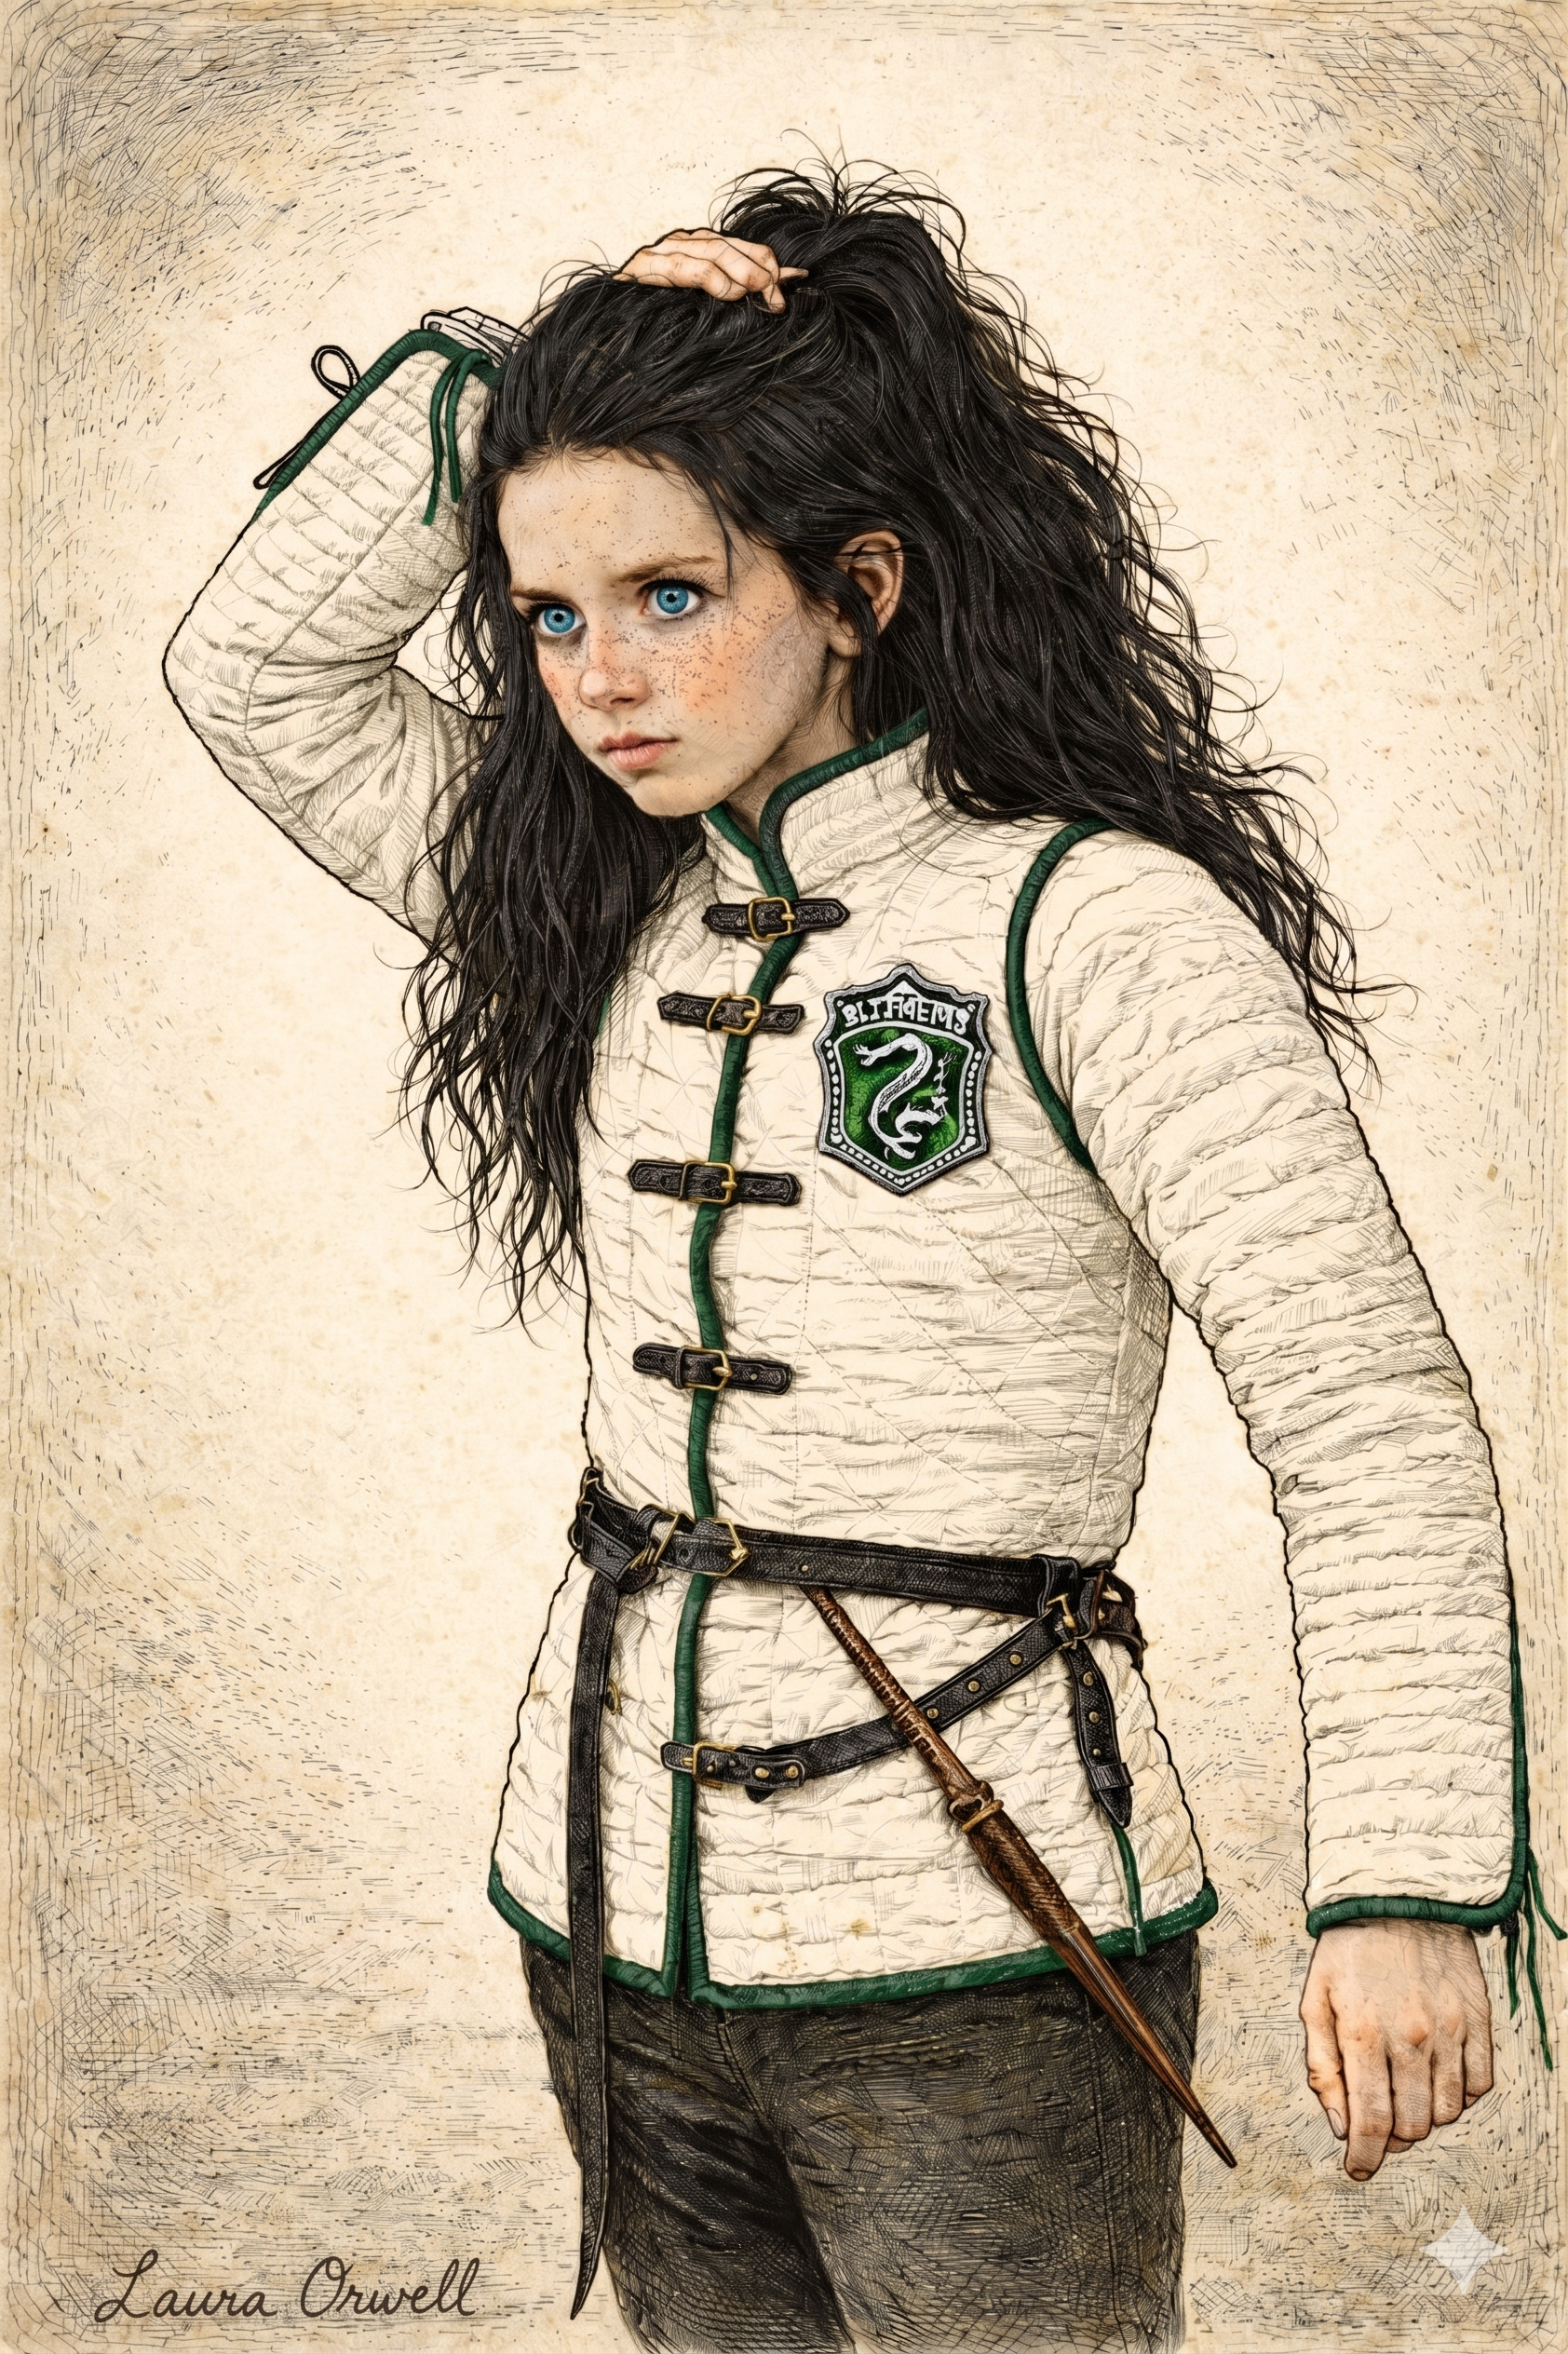
\includegraphics[width=0.49\textwidth]{images/fig_Laura_Orwell.png}
    \hfill
    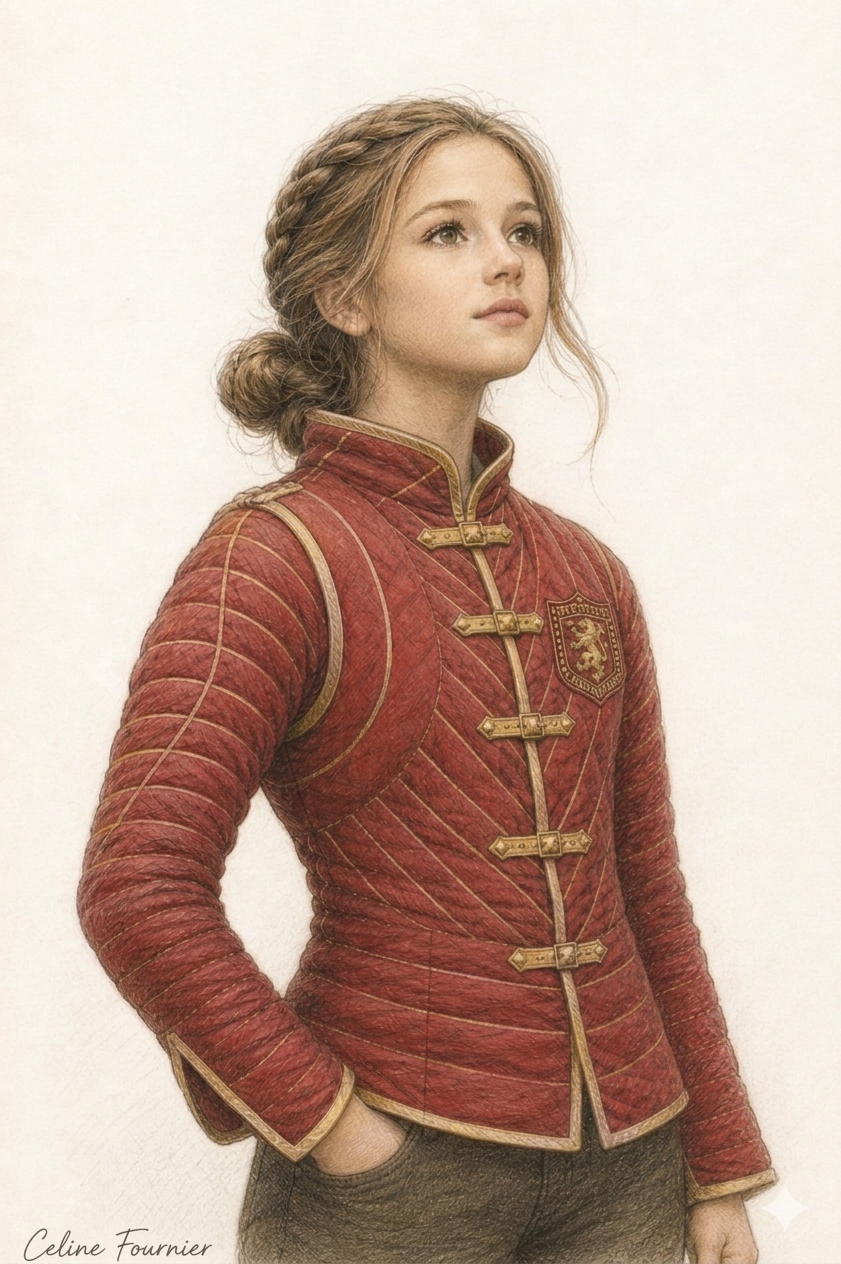
\includegraphics[width=0.49\textwidth]{images/fig_Celine_Fournier.png}
\end{figure}







\section*{Feather}
 
Professor Ligier arrived at None precisely.
 
He entered through the side door --- not the main entrance the students had used --- and crossed the room without greeting them. He was tall and lean, and he moved with a controlled, unhurried economy --- every gesture deliberate, nothing wasted, the habits of dangerous places worn into the body. His gambeson was a worn, creamy white with green edging along the front opening, collar, and cuffs, and a small Slytherin crest embroidered over the left breast. A wand sat at his left hip. A second --- shorter, thicker --- was strapped to his right forearm beneath the sleeve, visible only as a faint ridge against the quilted fabric.
 
He set a canvas satchel on the front desk and began unpacking it. Out came a wooden box the size of a bread loaf, a cloth bundle that clinked softly, a leather pouch, a small ceramic pot of black ink, a sheaf of parchment, and --- one by one, laid in a neat row --- a collection of long white feathers. He counted them without looking at the students, his lips moving slightly.
 
When the desk was arranged to his satisfaction, he picked up the feathers and walked the semicircle, placing one on the bench in front of each student. The feathers were goose quills, white, their shafts straight and their barbs undisturbed. 
 
He returned to the front of the room and stood with his hands at his sides.
 
\enquote{The only spell you will need today,} he said, \enquote{is \textit{Wingardium Leviosa}.}
 
His Latin was precise, clipped, and carried beneath it the low vowels of Norman French.
 
A murmur ran through the class. Several students exchanged looks of unmistakable relief --- a charm they had already practised, a spell with no sharp edges. Others, Aiko among them, looked faintly disappointed, their expectations of the Defence Against the Dark Arts classroom recalibrating downward with visible reluctance.
 
Ligier watched the murmur pass through the room and did not react to it.
 
\enquote{Trust me,} he said. \enquote{It will be more than enough for the first class.}
 
He drew his wand from his hip and held it over the feather he had kept for himself. He made the movements slowly, deliberately, exaggerating each component: the swish broad and theatrical, the flick sharp and high, the syllables drawn out so that every student in the room could hear the precise shape of each vowel.
 
\enquote{\textit{Win-GAR-dium Levi-O-sa}.}
 
The feather rose. It climbed smoothly from the desk, rotating once on its axis, and hung in the air at the level of Ligier's chest --- motionless, perfectly still, as though the air around it had thickened into glass.
 
He held it there for a moment. Then he lowered his wand and the feather drifted back down, as though it had nowhere else to be.
 
\enquote{Now you.}
 
The room filled with the sound of twenty wands being drawn from twenty new belt loops with varying degrees of confidence. Swishes cut the air. The syllables rose in an overlapping, slightly ragged chorus --- \textit{Wingardium Leviosa, Wingardium Leviosa} --- and across the semicircle, feathers began to move.
 
Six rose on the first attempt --- perhaps seven, depending on whether one counted Cassian's, which lifted two inches, drifted sideways, and settled back down gently. Laura Orwell's feather climbed without hesitation, as steady and controlled as Ligier's demonstration, and hung in the air at precisely the same height. Julian's rose with a fluid elegance that suggested the wand movement had been practised in front of a mirror.
 
Thomas's feather shot to the ceiling.
 
It left the desk like a crossbow bolt --- a white blur that covered the distance to the vaulted stone above in less than a second and struck the masonry with a faint, pathetic \textit{tick} before tumbling back down, spinning end over end, and landing on the floor three benches away from where it had started.
 
Nobody laughed. Several students glanced at Thomas, then at Ligier, then back at their own feathers.
 
Thomas retrieved the quill. He set it on the bench in front of him, adjusted his grip on his wand, and tried again.
 
The feather flew sideways. It crossed the width of the classroom in a flat, horizontal streak, passing over the heads of two Ravenclaws who ducked instinctively, and struck the far wall with a soft tap before drifting to the floor.
 
Thomas said nothing. His jaw tightened, very slightly, in a way that only Colum --- sitting beside him --- was close enough to notice.
 
By the time the rest of the class had achieved a stable levitation, Thomas was on his fourth attempt. The feather rose --- not gently, not smoothly, but it rose, and it held, trembling faintly in the air like a thing that was being restrained rather than lifted. It was not elegant. It was not still. But it was, by the definitions that mattered, levitating.
 
Ligier watched from the front of the room. His expression did not change.
 
\enquote{Good,} he said, when the last feather was airborne. \enquote{Now --- put your wands down.}
 
The feathers descended, one by one, as the students lowered their arms and placed their wands on the benches in front of them. The room went quiet, waiting for what came next. 
 
\enquote{The same spell,} Ligier said. \enquote{Without the wand.}
 
The silence deepened. Twenty students looked at their hands, then at their feathers, then at Ligier, then back at their hands.
 
Thomas raised his left hand. He did not think about it, precisely --- the motion was older than thought, something the body knew before the mind had time to interfere. He felt for the spell the way a musician feels for a note --- not by searching, but by knowing where it already was. His fingers opened, palm upward, and the feather rose.
 
It climbed smoothly, silently, and stopped. It did not tremble. It did not drift. It hung in the air above his palm with a stillness so absolute that it looked painted there --- more controlled, more certain, more completely \textit{his} than anything the wand had produced.
 
The room turned to look at him.
 
\enquote{Very good, Mr. Blackwood,} Ligier said. His tone was level, unimpressed in the way that suggested he had expected precisely this result and was merely confirming it. \enquote{The rest of you --- try.}
 
What followed was a slow, uneven accumulation of small successes. Colum's feather twitched. Astrid's rose an inch, hung for a heartbeat, and fell. Reza's drifted upward in a lazy, spiralling ascent that seemed to surprise him more than anyone. Celine managed a brief, wobbling hover that drew a gasp from herself and a quiet smile from Philippa, who had not yet moved her own feather at all but was observing everyone else's attempts with a cataloguing attention.
 
One by one, student after student, the feathers began to rise --- haltingly, briefly, without the clean authority of Thomas's effortless display, but rising nonetheless. Each success drew a small reaction from the students nearby --- a nod, a whispered word of encouragement, a grin.
 
Laura was the last.
 
She sat very still, her pale hands open in front of her, the feather resting on the bench undisturbed. Around her, feathers floated at various heights and with various degrees of stability, and her classmates were beginning to relax into the novelty of the thing. Laura's jaw was set, her blue eyes fixed on the quill with an intensity that was almost physical in its weight. She was not struggling visibly --- she was simply not succeeding, and for Laura Orwell, the distinction was meaningless.
 
The feather stirred. It rocked once on its shaft, then lifted --- barely, perhaps a finger's width above the wood --- and held. Her hands were rigid, her shoulders taut, and the effort was visible in a way it had not been with the wand. But it was done.
 
Ligier waited until she had held it for a full three seconds before he spoke.
 
\enquote{Good,} he said. The word carried no particular warmth, but neither did it carry pity, which was --- from Ligier --- perhaps the greater kindness.
 
He returned to the front desk and opened the wooden box.
 
Inside, arranged in cloth-lined compartments, were small geometric shapes --- cubes, spheres, triangles, cylinders --- carved from pale wood and polished smooth. He lifted out a second object: a flat board, roughly the size of a serving platter, into which matching holes had been cut. A cube-shaped hole, a round hole, a triangular slot, a cylindrical channel. The shapes and their corresponding openings were sized for small hands --- clearly, unmistakably, a children's toy.
 
He held it up.
 
\enquote{Using your wands,} he said, \enquote{place each shape through its corresponding hole.}
 
The reaction was immediate and unfavourable. A ripple of indignation passed through the class --- the particular offence of eleven-year-olds who have just been issued armour and belt-holstered wands being asked to play with an infant's puzzle. Hector's expression tightened with aristocratic disdain. Ewan opened his mouth to make a comment, reconsidered, and closed it again.
 
Ligier distributed the sets without acknowledging the mood. One box and one board per student. He waited until the last set had been placed, and then stepped back.
 
\enquote{Begin.}
 
Laura's wand moved with surgical precision. The first shape --- the cube --- rose from its compartment, rotated to align with the square opening, and dropped through with a clean, soft \textit{clack}. The sphere followed. Then the triangle, the cylinder, and the rest --- each one lifted, turned, and placed with speed and precision. The entire sequence took perhaps thirty seconds. She set her wand down and folded her hands in her lap.
 
It had looked almost easy.
 
Julian followed her --- his wand movements fluid and exact, the shapes rotating with a dancer's control. One by one, the rest of the class engaged with the task, and the indignation evaporated as they discovered that the children's toy was, in fact, considerably more difficult than it appeared. Levitating a feather required lifting a nearly weightless object straight up. Levitating a wooden cube, rotating it to the correct angle, and guiding it into a hole that was only slightly larger than the shape itself required something altogether different --- a continuous, three-dimensional awareness of the object's position, its orientation, and the precise amount of force being applied in each direction simultaneously.
 
Shapes clattered against boards, bounced off edges, and rolled across benches. Barnabus sent a sphere ricocheting off his board and into Mæve's lap. Celine's triangle refused to rotate and hung stubbornly in the air at the wrong angle, vibrating with the intensity of her focus.
 
Thomas destroyed the first box, and the second.
 
The cube lifted cleanly enough, but the force behind it was --- as with the feather --- disproportionate to the task. It struck the board at speed, punched through the square hole, split the wood beneath it, and embedded itself in the bench. Thomas looked at the damage, exhaled slowly, and raised his hand to request a replacement. The new board lasted longer. He managed the cube and the sphere before a misdirected cylinder cracked the board along the grain and sent two pieces spinning to the floor.
 
On the third set, he completed the task. It was not elegant. Several of the shapes bore the marks of impacts with the board's edges, and the final cylinder went through its hole with more force than finesse. But it was done.
 
When the last student had finished, Ligier collected his wand.
 
\enquote{Wandless.}
 
Thomas's hands moved before the word had finished settling. The cube rose from the box, turned in the air, and dropped through its hole with a precision that bordered on the mechanical. The sphere followed. Then the triangle, the cylinder, the rest --- each shape lifted, aligned, and placed with the same effortless fluency, his fingers making small, economical gestures that guided the objects as naturally as if he were touching them directly. The whole sequence was nearly as fast as doing it by hand.
 
He set his palms on the bench and waited.
 
Around him, the wandless attempts began. The results were --- predictably --- worse. Shapes drifted, wobbled, refused to rotate.
 
Laura's jaw was set again. The cube rose, slowly, unsteadily --- the control she commanded with a wand entirely absent from her bare hands. She guided it toward the board, overcorrected, and the cube veered left. She brought it back. It reached the opening, rotated --- too far --- and struck the edge. She tried again. The cube clipped the corner of the board and tumbled onto the bench.
 
She retrieved it with a sharp flick of her fingers and started over. This time, the triangle escaped her grip entirely and flew across the room in a flat arc, striking Ewan in the shoulder. The gambeson absorbed the impact without complaint. Ewan glanced down at his arm, then at Laura, and wisely said nothing.
 
More shapes flew. A cylinder bounced off Griffin's bench. A sphere rolled across the floor between Philippa's feet.
 
Laura finished last again. The final shape --- the cylinder --- dropped through its hole with a force that cracked the board's edge, and she sat back with an expression that dared anyone in the room to comment.
 
Nobody did.
 
Ligier walked to the front desk and opened the cloth bundle. Inside were needles --- long, sturdy sewing needles, each the length of a finger --- and spools of coarse thread. He laid them out in pairs.
 
Then he reached beneath the desk and produced a wooden crate. He opened it and lifted out a set of goggles --- heavy leather frames fitted with thick, clear glass lenses, the kind that a broom flyer might wear. He held them up.
 
\enquote{Put these on before you begin.}
 
The students took their goggles and fitted them over their eyes. The leather was stiff and smelled of tallow, and the lenses made the room slightly amber.
 
\enquote{Thread the needle,} Ligier said. \enquote{With your wand.}
 
The task was straightforward in description and excruciating in practice. The thread had to be lifted, straightened, guided through a hole barely wider than itself, and pulled through --- all at a distance of three feet, using only a wand. The margin for error was functionally zero.
 
Laura completed it on her first attempt. The thread rose from the spool, straightened into a rigid line, passed through the eye of the needle, and --- before anyone had quite registered what was happening --- looped back and tied itself into a small, neat knot. She set the needle down.
 
Thomas's thread hit the needle on the first attempt. Not the eye --- the shaft. The needle spun off the desk, flew point-first toward Griffin's bench, and struck the glass of his goggles with a sharp, bright \textit{ping} that drew a yelp of surprise and a very rapid reassessment of Ligier's decision to provide eye protection.
 
\enquote{Bloody hell,} Griffin said, touching the unscratched lens.
 
More needles flew. The room filled with the sound of small metallic impacts --- \textit{ping, tick, clink} --- as threads missed their targets and needles were launched from desks by misdirected force. Astrid's went straight up and stuck in the ceiling, where it remained for the rest of the lesson, glinting in the torchlight like a tiny stalactite.
 
The goggles earned their keep many times over.
 
When the wandless round came, the room had already accepted the pattern. Thomas threaded the needle on his first attempt --- the thread rising from the spool and passing through the eye with the same effortless, almost meditative control that characterised all his wandless work. Laura's thread refused to straighten. It curled, sagged, drifted sideways, approached the eye and missed, approached again and missed again. On her sixth attempt, it passed through, and she pulled it taut with a sharp, victorious motion that suggested the thread had been personally offensive to her.
 
The final task was a quill and ink.
 
Ligier placed a sheet of paper, a fresh quill, and a small ceramic pot of black ink in front of each student. The instruction was simple: dip the quill in the ink and write your name. With your wand.
 
The quill presented a new problem. Unlike the feather, which merely needed to rise, or the shapes, which merely needed to be placed, the quill required \textit{continuous, fine manipulation} --- a sustained, moving grip that had to lift, dip, and then trace letters with legible precision. It was, Thomas realised, as if Ligier had designed the entire afternoon as a single escalating argument: \textit{you think you can control this spell, and you cannot, and I will keep proving it until you believe me}.
 
Laura wrote her name in a clean, upright hand that could have passed for work done by her own fingers.
 
Thomas's first attempt sent the ink pot spinning across the desk. A plume of black ink erupted from the ceramic rim and arced through the air in a long, spectacular ribbon that caught the light from the windows beautifully before landing across the front of Barnabus's gambeson. The ink struck the quilted fabric and --- to the surprise of everyone except, presumably, William Taylor --- slid off it entirely, pooling on the bench beneath as though the surface of the gambeson were made of glass rather than cloth. The fabric remained perfectly, impossibly clean.
 
\enquote{Good gambesons resist dirt, these must be of the best quality} Philippa observed, looking down at the dark puddle on the bench with quiet satisfaction --- her earlier close examination of the garment vindicated.
 
More ink flew. The room became a study in aerodynamic chaos --- black droplets sailing in unpredictable arcs, quills dipping too deep and emerging trailing dark comets, parchments smeared beyond legibility. Barnabus dipped his quill, lifted it, and the entire contents of the ink pot followed --- a black, wobbling sphere of ink that hung in the air for one suspended, horrified moment before collapsing onto his paper, his bench, and his lap. The gambeson refused every drop.
 
Thomas wrote his name on the fourth attempt. The letters were legible, though a calligrapher would have had strong opinions about them.
 
The wandless round followed. Thomas wrote \textit{Thomas Blackwood} in a hand that was --- if not beautiful --- perfectly steady and entirely controlled. Laura's quill skittered across the parchment, leaving a trail that resembled a seismograph more than a signature. She finished, eventually. The \textit{L} was identifiable. The rest required good faith.
 
When the last student had completed the final task, Ligier returned the materials to the front desk with the same unhurried precision with which he had laid them out. The room was quiet --- not the nervous quiet of the lesson's beginning, but the settled quiet of twenty students who had been thoroughly, methodically humbled and were not entirely sure what to make of it.
 
Ligier stood at the front and looked at them.
 
\enquote{Before I can teach you Defence Against the Dark Arts,} he said, \enquote{I need you to be completely comfortable with your wands. Not competent. Not adequate. \textit{Comfortable}. I want the wand to feel as natural in your hand as a quill --- more natural, eventually. Most wizards cast spells the way most people write letters: with enough skill to be understood, but without any real mastery of the instrument. That is sufficient for most purposes.}
 
He paused.
 
\enquote{It is not sufficient for mine.}
 
He let the words settle. The anatomical diagrams on the wall --- the clinical illustrations of spell damage to human tissue --- seemed, in the silence, to grow slightly more vivid.
 
\enquote{I also want you to try the same spells without your wands,} he continued. \enquote{Most wizards are entirely defenceless the moment they are disarmed. I do not intend for that to be the case with my students.}
 
He folded his arms.
 
\enquote{But make no mistake --- a tool is always preferred to no tool. A wand is a precision instrument. It focuses, it channels, it multiplies. A wizard who can cast wandless is resourceful. A wizard who \textit{relies} on wandless magic when a wand is available is a fool.}
 
Thomas had the distinct sensation that Ligier was looking at him while making this remark. He kept his eyes forward and his expression neutral.
 
\enquote{Now,} Ligier said. \enquote{The fun part.}
 
Philippa, who had heard the phrase for the third time that day, thought privately that Hogwarts could be more creative with it's catchphrases.
 
\enquote{From this moment forward,} Ligier said, \enquote{I want your wands in your hands. Not on your belts. Not on your desks. In your hands. The wand should be the last thing you hold before you fall asleep at night and the first thing you reach for when you wake in the morning.  You will not, however, sleep with it --- not in your hand, not under your pillow. Nightmares and wands are a poor combination, and the castle has lost enough furniture over the centuries.You will eat with your wands. You will dress with your wands. You will open doors, carry books, and pour water with your wands. If a task can be done with magic, I want you to do it with magic. If it cannot --- hold the wand anyway.}
 
He looked at them --- twenty faces in amber-tinted goggles, ink-stained parchment in front of them, the residue of the afternoon's disasters still pooling on the benches beneath gambesons that had refused to absorb a single drop.
 
\enquote{You are dismissed, but keep your gambesons}.
 
Benches scraped. Students rose, stretched, compared their parchments, examined each other's gambesons for ink damage that did not exist. The mood was lighter than the lesson's content perhaps warranted --- the particular lightness that follows something demanding, when everyone has come out the other side with a story to tell.
 
Ligier's voice cut through the movement.
 
\enquote{Miss Orwell. Mr. Blackwood. Stay.}
 
The room emptied around them. Colum glanced at Thomas on his way out --- a look that carried a question and an offer simultaneously --- but Thomas shook his head, very slightly, and Colum went. Laura had not moved from her bench. She sat with her hands folded in her lap and her expression perfectly unreadable.
 
When the door had closed, Ligier crossed the room and stood in front of his daughter.
 
\enquote{Your wand,} he said.
 
Laura drew it and held it out. Ligier shook his head.
 
\enquote{Secure it on your belt.}
 
She slid the wand into the loop at her hip. Ligier reached into his satchel and produced a strip of linen cloth, pale and clean. He took Laura's right hand --- her wand hand --- and wrapped the cloth around her palm and fingers with practised efficiency --- quick, firm, the muscle memory of field dressings. When the hand was covered, he touched the cloth with his wand, and the linen stiffened, binding itself to her hand in a way that was clearly enchanted and clearly not coming off without the counter-spell.
 
Laura looked at her wrapped hand and said nothing. Her expression did not change, but something behind her eyes shifted --- a recognition, perhaps, that this was not punishment but something more complicated.
 
\enquote{Now you, Mr. Blackwood.}
 
Thomas stepped forward. Ligier nodded toward his wand.
 
\enquote{Draw it. Hold it in your left hand.}
 
Thomas drew his wand --- the dark, dense wood warm and familiar against his fingers. Ligier took another strip of linen and wrapped it around Thomas's hand and the wand together, binding the two into a single unit. The spell followed, and the cloth tightened. Thomas flexed his fingers experimentally. The wand was fixed in his grip --- not painfully, but absolutely. He could not release it without the charm being lifted.
 
Ligier stepped back and looked at Thomas.
 
\enquote{Wandless spells come naturally to you,} he said. His tone was not congratulatory. It was diagnostic --- the voice of a man identifying a condition. \enquote{That is unusual and it is valuable. But it is also, at this moment, a hindrance. Your wand work is poor because your instincts bypass it. Your body does not believe it needs the instrument, and so it fights the instrument, and you produce---} He gestured, vaguely, toward the ceiling, where Astrid's needle still glinted. \enquote{\textit{That}.}
 
Thomas said nothing. There was nothing to say.
 
Ligier turned to Laura.
 
\enquote{And you,} he said. His voice did not soften, exactly, but it lowered --- the slight modulation of a man speaking to his daughter while trying very hard to speak to his student. \enquote{I underestimated the effect of growing up at Hogwarts. You have spent eleven years surrounded by wands, watching wands, learning from wands. Your magic lives in the instrument. Without it---} He glanced at her wrapped hand. \enquote{Without it, you are starting from the beginning.}
 
Laura met his eyes. The blue of hers against the dark of his held for a moment --- the particular, loaded silence between a parent and child who understood each other well enough to argue without speaking.
 
\enquote{Unlike your classmates,} Ligier said, looking at both of them now, \enquote{you will not practise both wanded and wandless magic. Miss Orwell --- you will perform only wandless spells until I remove that binding. Mr. Blackwood --- you will perform only wanded spells until I remove yours.}
 
He paused.
 
\enquote{And I want you to teach each other.}
 
Laura looked at Thomas. Thomas looked at Laura. They wore the identical disapproval expressions of teenagers who has just smelled a fart --- a slow, involuntary horror that began at the nose and spread outward until it occupied the entire face.
 
Ligier, to his credit, did not smile. But the corner of his mouth moved --- once, briefly --- before settling back into its customary line.
 
\enquote{I am confident in your ability to do so,} he said. \enquote{You may go.}
 
They went. Laura turned left in the corridor. Thomas turned right. Neither looked back.
 
 \enquote{Bye Love.} Said professor Ligier to his daughter.
 
 \enquote{Bye daddy.} Said Laura do her father.


\section*{Wanded Banquet}
 
The castle bell struck six times, the deep, bronze voice of it rolling down through the stone corridors and settling into the bones of the building. Vespers. The sound reached the Defence Against the Dark Arts classroom through two feet of masonry and arrived diminished but unmistakable, cutting through the last of the post-lesson conversation like a blade through cloth.
 
Thomas flexed his left hand --- or tried to. The wand was still there, bound tight against his palm and fingers by Ligier's linen strip, the enchanted fabric warm and immovable. Across the corridor, Laura emerged from the classroom with her right hand held slightly away from her body, the wrapped fist carried with the careful, self-conscious rigidity. They did not speak. They walked in the same direction because the Great Hall was in the same direction, and for no other reason that either of them would have admitted to.
 
The first thing Thomas noticed, as they descended the main staircase with the general flow of students heading toward supper, was the goggles.
 
A group of fourth-years was crossing the entrance hall ahead of them, and every one of them was wearing heavy leather-and-glass goggles pushed up onto their foreheads. They were laughing --- the warm, knowing laughter of people heading into something they remembered very well. One of them caught Thomas's eye, glanced at his gambeson, and grinned in a way that was equal parts welcome and condolence.
 
Then Thomas saw the armour.
 
A sixth-year boy was descending the opposite staircase in a full suit of plate armour --- breastplate, pauldrons, vambraces, greaves, the works --- polished to a theatrical shine and worn over what appeared to be his school robes. His visor was up. He was eating an apple. Beside him, a girl in a gambeson and goggles was shaking her head slowly, but she was smiling. Further along the corridor, two more older students clanked past in mismatched pieces of armour --- one wearing a single gauntlet on his left hand and nothing else of note, the other in a full chainmail hauberk that reached his knees and produced a continuous, silvery rustling as he walked.
 
\enquote{Is that ---} Laura began.
 
\enquote{I think so,} Thomas said.
 
They entered the Great Hall.
 
The four long house tables were dressed in their usual arrangement --- bare oak, no tablecloths, the wood dark and scarred from centuries of use. Tablecloths, as every student learned in their first week, were reserved for ceremonial occasions: the Sorting Feast, the end-of-year banquet, and certain holidays. Ordinary meals were served on the naked wood, and the wood bore the evidence of it.
 
But the seating was not ordinary.
 
At the near end of the hall, a full section of one of the long tables had been set apart --- separated from the nearest older students by a good thirty metres of empty bench --- twenty places had been laid. Not Gryffindor places, not Hufflepuff places, not Ravenclaw or Slytherin places. Twenty places, together, for twenty first-years.
 
No house colours marked the section. No banners hung above it. It was simply a stretch of table with plates and cups and the implicit understanding that whoever sat there belonged to each other before they belonged to their houses.
 
The first-years arrived in ones and twos and small, mixed clusters --- Gryffindors walking with Ravenclaws, Hufflepuffs beside Slytherins, the house boundaries that had been drawn the night before already softened by a single day of shared classes. Colum and Thomas reached the table together and sat near the centre. Celine slid onto the bench across from them, Philippa beside her. Baldwin appeared at Colum's shoulder, spectacles slightly askew behind the goggles. Barnabus arrived eating something he had apparently obtained between the third floor and the ground floor by means that remained unclear.
 
Laura, after a moment's hesitation that was brief enough to be almost invisible, took the place on the bench to Thomas's left.
 
They were still wearing their gambesons and goggles. Everyone was.
 
Colum looked at the reserved section --- the twenty places, all houses together, the empty gap between them and the older students. He looked at the older students in their armour and goggles, thirty metres away, laughing. He looked at the quantity of food that was being laid out in front of them.
 
\enquote{Thomas,} he said quietly.
 
\enquote{I see it.}
 
The platters arriving at the first-year section were enormous. Meat pies --- whole ones, their crusts golden and steaming --- were set down in a row that stretched the full length of the reserved section. Behind them came trenchers of roasted root vegetables, baskets of bread, bowls of thick gravy, crocks of butter, wheels of cheese, dishes of honeyed fruits, and --- conspicuously, almost aggressively --- a towering arrangement of cakes, tarts, and pastries that occupied the centre of the table like a sugary fortress. Thomas counted the platters. He looked at the twenty first-years around him. He looked back at the food. The ratio was absurd --- three times what the older students had received at their distant end of the hall, perhaps more.
 
An hour past Vespers, the plates, glasses, and silverware had been distributed and the last of the serving platters had found their positions. At the far end of the tables, the older students had begun eating with the unhurried composure of people who knew what was coming and were in no particular rush to begin it. Several of them had turned in their seats to watch the first-year section with undisguised anticipation. A second-year girl in a Ravenclaw gambeson was whispering urgently to the boy beside her, both of them grinning.
 
At the high table, Headmaster Hepburn rose. He did not amplify his voice. He did not need to --- the hall had gone quiet on its own, the particular expectant silence of a room that knows it is about to be given permission.
 
Hepburn smiled. It was the smile of a man who had presided over this moment for more years than most of the students had been alive, and who had not tired of it.
 
He drew his wand, pointed it at a single sheet of paper on the table before him, and tapped it once. The paper shivered, split, and multiplied --- one became two, two became four, four became eight, the sheets dividing with the quiet, urgency of a thing that had somewhere to be. Twenty small squares of paper now sat in a neat stack. Hepburn tapped the stack again, and each square folded itself --- rapidly, precisely --- into the shape of a small owl. Twenty paper owls sat on the high table, their creased wings held at angles that suggested flight was imminent and patience was not their strong suit.
 
Hepburn flicked his wand. The owls launched.
 
They crossed the hall in a wheeling, rustling flock, banked sharply over the Ravenclaw table --- drawing a collective flinch from two second-years who remembered their own year too well --- and descended upon the first-year section. Each owl found its target, landing on the bench or the table or, in Barnabus's case, directly on top of his head, and then tore itself apart with a decisive rip that left the message exposed and the delivery mechanism in small, fluttering pieces.
 
Thomas picked up his fragment of paper. The handwriting was Hepburn's --- large, round, and warm, the script   wrote the way he spoke.
 
\begin{quote}
\textit{The wanded banquet: for you to eat using your wands. It is, though, an excellent opportunity --- and excuse --- to throw, by mistake of course, a cake in the face of an esteemed colleague who needs more sugar in his life. Let the food wars begin.}
\end{quote}
 
The hall held its breath for exactly one second.
 
Then Barnabus Finch, who had not finished reading the note but had already identified the nearest meat pie, drew his wand and bellowed \enquote{\textit{Wingardium Leviosa}!} with the full-throated conviction of a boy who had been waiting his entire life for official permission to throw food.
 
The pie rose. It did not rise well --- it wobbled, tilted, and shed a quantity of gravy onto the table --- but it rose, and the sight of it airborne was all the catalyst the room required.
 
Nineteen wands came out. The air filled with incantations, with the crack of levitation charms and the wet, heavy sound of food in unpredictable motion. A bread roll sailed past Philippa's ear. A wedge of cheese described a slow, tumbling arc and struck Baldwin squarely in the chest, leaving a yellow smear across his gambeson that the fabric refused to absorb. From down the table, a tart rose with impressive stability and deposited itself --- with what could only be described as gentle precision --- on the top of Julian Beauchamp's perfectly arranged hair.
 

%Julian closed his eyes. He sat very still for a moment, blackberry filling running slowly down his temple, and then --- with the careful, wounded dignity of a boy who had spent twenty minutes arranging his hair before supper --- he wiped his face with the back of his hand, examined the purple smear on his fingers, and sighed the sigh of a man who had known, on some level, that this was coming and had chosen to sit here anyway.

At the far end of the hall, the older students erupted in cheers.
 
Thomas looked at the chaos. He looked at the meat pie in front of him. He looked at the wand bound to his left hand.
 
He raised the wand, focused on a wedge of pie, and spoke the incantation carefully. \enquote{\textit{Wingardium Leviosa}.}
 
The wedge of pie left the plate like a stone from a catapult. It crossed thirty metres of open hall in a flat, screaming trajectory, trailing gravy and pastry fragments, and struck the invisible barrier of a \textit{Protego} charm with a wet, percussive \textit{thwack} that silenced the nearest tables. A fourth-year student --- tall, dark-haired, wand raised --- stood behind the shimmering shield, pie debris sliding slowly down its surface.
 
\enquote{Good arm,} the fourth-year called out, lowering his shield. \enquote{Terrible aim.}
 
Laura, sitting beside Thomas, had watched the entire sequence with her wrapped right hand resting on the table and an expression that was working its way through disbelief toward something closer to clinical fascination.
 
\enquote{How,} she said, slowly, \enquote{can someone be so adept at wandless spells and so completely useless with a wand?}
 
Thomas set his bound wand hand on the table. \enquote{You try, then.}
 
Laura looked at him. She looked at the pie. She raised her left hand --- her unbound hand, the one that had never carried a wand, the one that Ligier had left free precisely because it had never been her instrument --- and focused.
 
A second wedge of meat pie rose from the plate. It wobbled. It drifted. It made a valiant attempt at a controlled trajectory toward the older students. Then the control slipped, the wedge accelerated, and it sailed across the hall in a long, curving arc that bore no resemblance to its intended flight path and struck the same fourth-year squarely on the shoulder.
 
\enquote{\textit{Protego},} the boy said, far too late. He looked down at his shoulder. He picked up the piece of pie that had landed on his gambeson, examined it with a thoughtful expression, took a bite, and announced to the hall at large: \enquote{Not bad. Not bad at all.}
 
Laura lowered her hand. Her jaw was tight, but there was a flicker in her blue eyes that might, in better light, have been the beginning of a reluctant smile.
 
She turned to Thomas. \enquote{Using a wand,} she said, \enquote{is like writing with a quill. Or eating a pudding with a spoon. You could do both with your bare hands, but it would be a mess, wouldn't it?}
 
Thomas considered this. \enquote{And wandless magic,} he said, \enquote{is like eating a chicken leg with bare hands. You could do it with a fork and a knife, but it would be a mess, wouldn't it?}
 
Laura looked at him for a long moment. The corner of her mouth moved --- once, briefly --- before settling back into its customary line.
 
\enquote{Fair,} she said.
 
Something shifted between them. Not warmth, exactly --- neither of them was built for easy warmth with strangers --- but the particular, grudging clarity that comes when two people who are very good at different things recognise that the other's skill is not an insult to their own but a mirror of their own deficit, held up without malice, in language that left nothing to be misunderstood.
 
\enquote{Show me your grip,} Laura said, nodding toward his bound hand.
 
Thomas raised his left hand, the wand fixed in its linen binding. Laura studied it with the focused, assessing gaze of a girl who had held a wand since she could walk and understood its mechanics the way a carpenter understands the grain of wood.
 
\enquote{You're holding it like a weapon,} she said. \enquote{You're bracing against it. It's not fighting you --- you're fighting it. The shaft should rest here ---} she indicated the base of his fingers with her free hand --- \enquote{and the pressure comes from here, the thumb pad. Not the fist. The wand is not a hammer, Thomas. It is a quill.}
 
Thomas adjusted. The difference was small --- a fraction of an inch in the pressure, a slight loosening in the grip --- but when he pointed the wand at a bread roll and spoke the incantation, the roll rose from the plate with a smoothness that was, by the standards of the evening, almost graceful. It wobbled. It drifted slightly left. But it did not rocket across the hall like a siege projectile, and when he set it down on the table, it landed rather than crashed.
 
\enquote{Better,} Laura said. She did not elaborate. From Laura, the absence of criticism was the compliment.
 
\enquote{Your turn,} Thomas said. \enquote{Open your hand. Not like a claw --- flat. The magic doesn't need to be gripped. It needs to be directed. Think of it like pointing at something. You don't grab the air between you and the thing; you just ---} he extended his right hand, fingers straight, palm down --- \enquote{indicate.}
 
Laura uncurled her left hand. She held it over a small pastry, fingers extended, and focused. The pastry trembled. It rose --- barely, an inch perhaps --- and hung in the air with a concentration of effort that was visible in the tendons of Laura's wrist. Then it fell.
 
\enquote{Again,} Thomas said. \enquote{Flatter hand. Less force. You're pushing the spell out like a shove. It needs to be a breath.}
 
Laura tried again. The pastry rose higher this time --- three inches, then four --- and held. It was not steady. It was not elegant. But it was sustained, and when she lowered her hand, the pastry descended rather than dropped.
 
\enquote{A breath,} she repeated, turning the word over.
 
Thomas nodded. \enquote{With a wand, you're writing each letter of the spell. Without one, you're saying the whole word at once. You don't need to pronounce each sound --- you just need to mean it.}
 
The food war continued around them, but they had drifted to the edge of it --- two students sitting side by side amid the cheerful carnage, passing food back and forth, each attempt a lesson. Laura would say something precise about wrist angle or follow-through, and Thomas's next charm would be marginally less violent. Thomas would describe the feeling of wandless casting in terms that were intuitive rather than technical --- weight, temperature, direction --- and Laura's next attempt would hold a fraction of a second longer.
 
There were mistakes. Thomas sent a gravy boat spinning across the table and into Mæve's lap. Laura's attempt to levitate a bread roll produced a sharp sideways lurch that deposited it in Cassian's cup, which Cassian accepted with the equanimity of a boy who had seen stranger things fall from the sky tonight.
 
And there were \textit{mistakes} --- the kind that arrived with suspicious frequency and unerring accuracy at the exact position of Julian Beauchamp's hair. A dollop of custard, launched by Thomas in what was ostensibly an exercise in controlled trajectory. A fragment of fruit tart, directed by Laura in what she described, with perfect composure, as \enquote{a calibration attempt.} A small, beautifully aimed sphere of mashed turnip that neither of them claimed responsibility for and that landed with a soft, definitive \textit{plop} on the crown of Julian's head, where it sat like a pale, savoury beret.
 
\enquote{His hair,} Laura observed, with the clinical detachment of a naturalist documenting a species under stress, \enquote{is remarkably absorbent.}
 
\enquote{It's a gift,} Thomas agreed.
 
Elsewhere along the table, the banquet had found its rhythm. Colum and Ewan, the two Scots, had enlisted the French — Celine and Philippa — against the English: Hector, Griffin, Cassian, and Efe — who protested but was deemed English enough.
 
Aiko, further along the bench, was levitating a single grape with surgical focus --- waiting, motionless, for the precise moment when her target opened his mouth to speak, and then launching it. She had a hit rate that was, by the end of the evening, genuinely alarming. Griffin had laid three different wands on the table beside an assortment of food and was conducting what appeared to be a systematic trial of which wand threw which food best, a project that produced inconsistent results and a great deal of collateral damage.
 
At the high table, Headmaster Hepburn had produced his own plate of food and was eating with the serene contentment of a man surveying a battlefield that was going exactly as planned. Beside him, Professor Ravenclaw sat in perfect, untouched stillness, her robes immaculate, her expression suggesting that she had opinions about the proceedings that she was choosing, with considerable restraint, not to share. Professor Grim was watching the first-year section with quiet attention, his eyes moving from student to student, cataloguing. Professor Ligier was not present; his chair was empty. Professor Millan was present but had apparently decided that the floor was a better vantage point than the table --- she was sitting cross-legged on the flagstones near the end of the high table, eating a bread roll and watching the food fly with the bright, appreciative eyes of a woman who fundamentally approved of chaos conducted in good spirits.
 
The evening deepened. The enchanted ceiling shifted from the pale amber of late afternoon through the long, slow graduation of dusk --- indigo creeping in from the edges, the first stars appearing, the golden constellations beginning their nightly transit across the painted heavens.
 
Gradually, the food war ebbed. The ammunition diminished. The trajectories grew lazier, the impacts softer, the laughter quieter. The gambesons, which had taken the full brunt of the evening without complaint, were spotted and streaked with the evidence of a hundred direct hits --- gravy, custard, honey, cheese, fruit, and at least one substance that defied identification --- and yet the fabric beneath was clean, the quilted surface shedding every drop and stain as though the mess were happening to someone else. The goggles, which had seemed excessive at the start of the evening, had earned their keep many times over; Thomas counted at least four occasions on which his lenses had intercepted something that would otherwise have required medical attention.
 

 
In the quiet that followed the last of the flying food, Thomas sat with his bound hand resting on the oak table and looked at the wand. Three hours ago, every spell he cast with it had been a small explosion --- too much force, too little control, the magic surging through the wood like water through a pipe that was too narrow for the pressure behind it. Now, the last bread roll he had levitated had risen smoothly, traveled in a controlled arc, and landed --- more or less --- where he had intended it to land. The improvement was not dramatic. It was not mastery. But it was real, and he could feel the difference in his wrist and his fingers --- a looseness that had not been there before, a willingness to let the wand lead rather than forcing it to follow.
 
Beside him, Laura was turning a small apple over in the air above her open left palm. It rotated slowly, steadily, the wandless magic sustaining it with a patience that would have been impossible at the start of the evening. Her face was tight with concentration, but the effort was no longer the clenched, whole-body strain it had been during Ligier's lesson. Something had unlocked. The apple hung in the air like a thing that belonged there.
 
She set it down on the table, gently.
 
Neither of them said anything about the improvement. Neither of them needed to.
 
The castle bell struck nine times --- Compline --- and the sound was quieter than it had been in the morning, somehow, as though the bell itself had softened with the hour, its bronze voice muffled by the weight of the night above. The enchanted ceiling had long since settled into its fullest darkness, the golden constellations of Orion and Cassiopeia sliding slowly across the heavens, the silver  faint and steady.
 
From the high table, Hepburn rose. He looked out across the hall --- the older students at their distant end, the twenty first-years in their single, shared section, the whole room sticky and satisfied and thoroughly, completely happy --- and he smiled the smile of a man who had seen this same scene play out for decades and had not once grown tired of it.
 
\enquote{Clean yourselves up,} he said. \enquote{The prefects' baths have been prepared --- all seven of them --- steam already rising, for those who wish to rid their hair of blueberry, custard, or worse before bed.} He paused, his gaze drifting, with the faintest suggestion of intent, toward Julian. \enquote{Sleep well.}
 
They went. But not immediately, and not by house. They went the way the ship had taught them to go --- together at first, lingering in the entrance hall, reluctant to split into four directions when they had just spent an evening being one thing. Celine was still laughing about something Barnabus had said. Colum's ears were still red from a direct hit with a custard tart that Ewan had landed from an improbable distance. Philippa walked beside Mæve, the two of them discussing something in low, serious voices that were entirely at odds with the gravy stains on their gambesons. Cassian was looking up at the real sky through the open doors, comparing it to the enchanted ceiling he had just left. Elara's sketchbook was tucked under her arm, and even in the torchlight of the entrance hall, Thomas could see that the page she had been working on was full --- figures in gambesons, flying food, the warm chaos of the evening rendered in charcoal and ochre.
 
 Eventually, the group began to thin—but not in the way it usually did. Instead of turning off toward their respective houses, they drifted together through the corridors and up the staircases, following a shared, unspoken direction, until they reached the door that led to the prefects’ baths.

Someone murmured the password. The door yielded.

Inside, warmth and steam spilled out to meet them. Beyond lay not a single chamber, but a succession of bathing rooms, each already prepared—water drawn, taps gleaming faintly in the haze, the air thick with heat.

For a moment, they lingered at the threshold, as though uncertain how to undo the evening’s strange unity.

Then, gradually, they arranged themselves—not by house, but by simple necessity: by gender, by space, by who fit where. Conversations continued, split and softened by walls and steam, but not entirely broken.

The evening loosened its grip, little by little, as laughter gave way to quieter voices and the work of washing away blueberry, custard, and the rest.

On his shoulder, an owl-shaped piece of parchment—one of Hepburn’s enchanted notes, slightly crumpled, slightly gravy-stained—fluttered once in the warm air, as though remembering that it had once known how to fly, and then was still.
 
Eventually, the group began to form again. Cecile touched Celine's shoulder --- a brief, gentle gesture --- and headed toward the Hufflepuff corridor, Baldwin and Barnabus falling into step beside her. Cassian and Ewan turned toward the Ravenclaw tower, still arguing amicably about something. Aiko descended the steps toward the dungeons without a word, her posture immaculate, her gambeson spotless.
 
Thomas reached the foot of the grand staircase. Laura was heading in the opposite direction, toward the Slytherin common room. At the point where their paths diverged, she stopped.
 
\enquote{At Terce tomorrow?} she said, without turning around.
 
Thomas paused on the first step. \enquote{The breakfast?}
 
\enquote{The practice.}
 
He looked at her --- the wrapped hand, the dark hair, the straight back, the absolute refusal to frame the request as anything other than a practical arrangement between two people who had something the other needed.
 
\enquote{At Terce} he said.
 

 


























































